\begin{figure}[htbp]
    \centering
    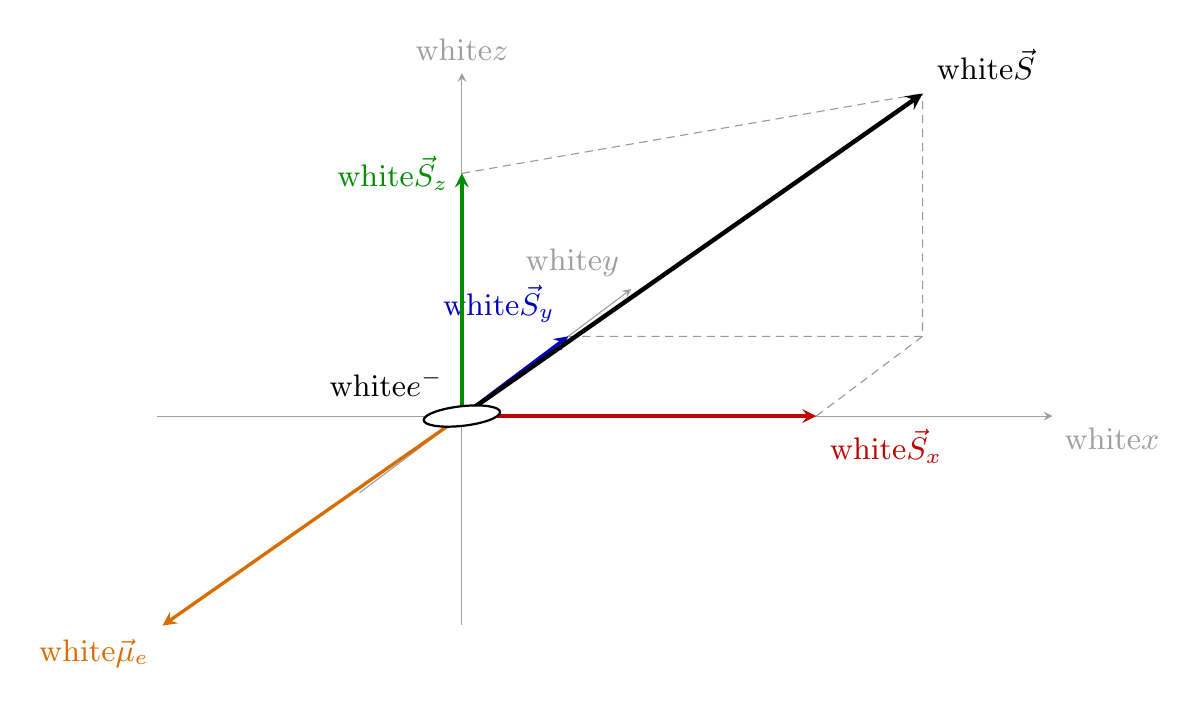
\begin{tikzpicture}[>=stealth, scale=1.25, transform shape, every node/.style={font=\small}, x={(2cm,0cm)}, y={(0.8cm,0.6cm)}, z={(0cm,1.7cm)}]
        \coordinate (O) at (0,0,0);
        \coordinate (X) at (1.8,0,0);
        \coordinate (Y) at (0,1.35,0);
        \coordinate (Z) at (0,0,1.45);
        \coordinate (S) at (1.8,1.35,1.45);

        \draw[->,gray!75] (-1.55,0,0) -- (3.0,0,0) node[below right] {\contour{white}{$x$}};
        \draw[->,gray!75] (0,-1.3,0) -- (0,2.15,0) node[above left] {\contour{white}{$y$}};
        \draw[->,gray!75] (0,0,-1.25) -- (0,0,2.05) node[above] {\contour{white}{$z$}};

        \draw[->,very thick,red!75!black] (O) -- (X)
            node[below right] at (X) {\contour{white}{$\vec{S}_x$}};
        \draw[->,very thick,blue!75!black] (O) -- (Y)
            node[above left] at (Y) {\contour{white}{$\vec{S}_y$}};
        \draw[->,very thick,green!55!black] (O) -- (Z)
            node[left] at (Z) {\contour{white}{$\vec{S}_z$}};
        \draw[densely dashed,gray!80] (X) -- (1.8,1.35,0) -- (S);
        \draw[densely dashed,gray!80] (Y) -- (1.8,1.35,0);
        \draw[densely dashed,gray!80] (Z) -- (S);
        \draw[->,ultra thick,black] (O) -- (S)
            node[above right] at (S) {\contour{white}{$\vec{S}$}};
        \draw[->,very thick,orange!85!black] (O) -- (-1.17,-0.8775,-0.9425)
            node[below left] at (-1.17,-0.8775,-0.9425) {\contour{white}{$\vec{\mu}_e$}};
        \filldraw[fill=white,draw=black,thick] (O) circle (0.18);
        \node[above left=2pt] at (O) {\contour{white}{$e^{-}$}};
    \end{tikzpicture}
    \caption{Esquema tridimensional de un electrón, el espín $\vec{S}$ y sus componentes $\vec{S}_x$, $\vec{S}_y$ y $\vec{S}_z$ en los ejes coordenados; el momento magnético $\vec{\mu}_e$ apunta en sentido opuesto, pues $\vec{\mu}_e=-g_e\mu_B\vec{S}/\hbar$, con $\mu_B=e\hbar/(2m_e)$. Para un electrón de espín $1/2$, cada componente medida puede tomar $S_i=\pm\hbar/2$. La descomposición dibujada es esquemática: las componentes no pueden medirse simultáneamente, ya que $[\hat S_i,\hat S_j]\ne0$ para $i\ne j$.}
    \label{fig:electron-sg}
\end{figure}